\documentclass[a4paper,11pt]{article}

% \usepackage[smartEllipses]{markdown}
% \usepackage[hashEnumerators,smartEllipses]{markdown}
% \usepackage[hashEnumerators,smartEllipses,hybrid]{markdown}
\usepackage[hybrid]{markdown}
\usepackage[export]{adjustbox} % рамки вокруг фото
\usepackage{minted} % Для вставки кода
% \usepackage{xpatch}
% \xpretocmd{\inputminted}{\par\vspace{1em}}{}{}
% \xapptocmd{\inputminted}{\par\vspace{1em}}{}{}
% \usepackage{indentfirst}
% \setlength{\parindent}{0pt} % Отключает отступ в начале каждого абзаца
\usepackage{parskip} % убрать красную строку и добавить вертикальный отступ между абзацами


%%% Мои команды
\newcommand{\insertMyCode}[2]{ % вставка кода
    % #1 — язык
    % #2 — путь до файла
    \inputminted[
    % framesep=2mm,
    baselinestretch=1.2,
    bgcolor=LightGray!30,
    fontsize=\footnotesize,
    linenos
    ]{#1}{#2}
}


%%% Работа с русским языком
\usepackage{cmap} % поиск в PDF
\usepackage{mathtext} % русские буквы в фомулах
\usepackage[T2A]{fontenc} % кодировка
\usepackage[utf8]{inputenc} % кодировка исходного текста
\usepackage[english,russian]{babel} % локализация и переносы

%%% Дополнительная работа с математикой
\usepackage{amsmath,amsfonts,amssymb,amsthm,mathtools} % AMS
\usepackage{icomma} % "Умная" запятая: $0,2$ —- число, $0, 2$ —- перечисление

%%% Перенос знаков в формулах (по Львовскому)
\newcommand*{\hm}[1]{#1\nobreak\discretionary{}
{\hbox{$\mathsurround=0pt #1$}}{}}

%%% Работа с картинками
\usepackage{graphicx} % Для вставки рисунков
\graphicspath{{images/}} % папки с картинками
% \setlength\fboxsep{3pt} % Отступ рамки \fbox{} от рисунка
% \setlength\fboxrule{1pt} % Толщина линий рамки \fbox{}
% \usepackage{wrapfig} % Обтекание рисунков текстом

%%% Работа с таблицами
\usepackage{array,tabularx,tabulary,booktabs} % Дополнительная работа с таблицами
\usepackage{longtable} % Длинные таблицы
\usepackage{multirow} % Слияние строк в таблице

%%% Теоремы
% \theoremstyle{plain} % Это стиль по умолчанию, его можно не переопределять.
\newtheorem{theorem}{Теорема}[section]
\newtheorem{proposition}[theorem]{Утверждение}

\theoremstyle{definition} % "Определение"
\newtheorem{corollary}{Следствие}[theorem]
\newtheorem{problem}{Задача}[section]

\theoremstyle{remark} % "Примечание"
\newtheorem*{nonum}{Решение}

%%% Программирование
\usepackage{etoolbox} % логические операторы

%%% Страница
% \usepackage{extsizes} % Возможность сделать 14-й шрифт % конфликт с parskip
\usepackage{geometry} % Простой способ задавать поля
\geometry{top=25mm}
\geometry{bottom=35mm}
\geometry{left=20mm}
\geometry{right=20mm}

\usepackage{fancyhdr} % Колонтитулы
\pagestyle{fancy}
\renewcommand{\headrulewidth}{0mm} % Толщина линейки, отчеркивающей верхний колонтитул
% \lfoot{Нижний левый}
% \rfoot{Нижний правый}
% \rhead{Верхний правый}
% \chead{Верхний в центре}
% \lhead{Верхний левый}
\cfoot % По умолчанию здесь номер страницы

\usepackage{lastpage} % Узнать, сколько всего страниц в документе.

\usepackage{soul} % Модификаторы начертания

\usepackage{setspace} % Интерлиньяж
%\onehalfspacing % Интерлиньяж 1.5
%\doublespacing % Интерлиньяж 2
%\singlespacing % Интерлиньяж 1

\usepackage{hyperref}
\usepackage[usenames,dvipsnames,svgnames,table,rgb]{xcolor}
\hypersetup{ % Гиперссылки
unicode=true, % русские буквы в раздела PDF
pdftitle={Заголовок}, % Заголовок
pdfauthor={Автор}, % Автор
pdfsubject={Тема}, % Тема
pdfcreator={Создатель}, % Создатель
pdfproducer={Производитель}, % Производитель
pdfkeywords={keyword1} {key2} {key3}, % Ключевые слова
colorlinks=true, % false: ссылки в рамках; true: цветные ссылки
linkcolor=red, % внутренние ссылки
citecolor=green, % на библиографию
filecolor=magenta, % на файлы
urlcolor=cyan % на URL
}

\usepackage{multicol} % Несколько колонок

%%% Хз что это (потом разобраться)
% \usepackage{upgreek}
\usepackage{cite}
\usepackage{csquotes} % Еще инструменты для ссылок
%Смотри источник 1 \cite{qwerty,Fama,Fama2}.
%\renewcommand{\refname}{Список источников}  % По умолчанию %"Список литературы" (article)
%\renewcommand{\bibname}{Литература}  % По умолчанию "Литература" (book и report)
%\renewcommand{\familydefault}{\sfdefault} % Начертание шрифта

\begin{document}


\begin{titlepage} % начало титульной страницы
\pagestyle{empty}
\begin{center}

\Large
\textbf{Федеральное государственное автономное образовательное учреждение высшего образования\\
«Национальный исследовательский университет\\
«Высшая школа экономики»}\\
\vspace{5mm}

\Large
Образовательная программа \\
«Прикладная математика»
\vspace{40mm}

\Large
\textbf{ОТЧЕТ} \\
\textbf{По лабораторной работе № 3} \\
\vspace{5mm}
\Large По предмету \\
\LARGE\textbf{«Численные методы»} \\
\vspace{5mm}
\Large По теме \\
\LARGE\textbf{«Решение систем алгебраических уравнений итерационными методами»}
\end{center}

\begin{center}
\vfill

\large
\begin{flushright}
\textbf{Выполнил} \\
студент группы БПМ211 \\
Кудряшов Максим Дмитриевич \\
\end{flushright}

\large
\begin{flushright}
\textbf{Проверил} \\
Брандышев Петр Евгеньевич \\
\end{flushright}

\large
\vspace{20mm}
Москва - 2024
\end{center}
\end{titlepage} % конец титульной страницы

\newpage
\tableofcontents
\newpage

\section{Метод Ньютона (№ 4.1.8)}

\subsection{Формулировка задания}

Найти с точностью $\epsilon = 10^{-6}$ все корни системы нелинейных уравнений:
$$f_1(x_1,x_2)=0$$
$$f_2(x_1,x_2)=0$$
Использовать метод Ньютона для системы нелинейных уравнений, найти корни с помощью встроенного функционала решения уравнений.

1. Используя встроенные функции, локализовать корни системы уравнений графически.

2. Написать программу-функцию, вычисляющую корень системы двух нелинейных уравнений по методу Ньютона с точностью $\varepsilon$. Предусмотреть подсчет количества итераций. Для решения соответствующей системы линейных алгебраических уравнений использовать встроенную функцию.

3. Используя написанную программу, вычислить все корни заданной системы с точностью $\varepsilon$

4. Используя встроенные функции, найти все корни системы с точностью $\varepsilon$. Сравнить с результатами, полученнными в п. 3.


\subsection{Код на Python}

\subsubsection{Построение графика}

\insertMyCode{python3}{../create_plot.py}

\subsubsection{Решение системы методом Ньютона}

\insertMyCode{python3}{../newton_method.py}

\newpage
\subsection{Результаты}

\begin{figure}[h]
    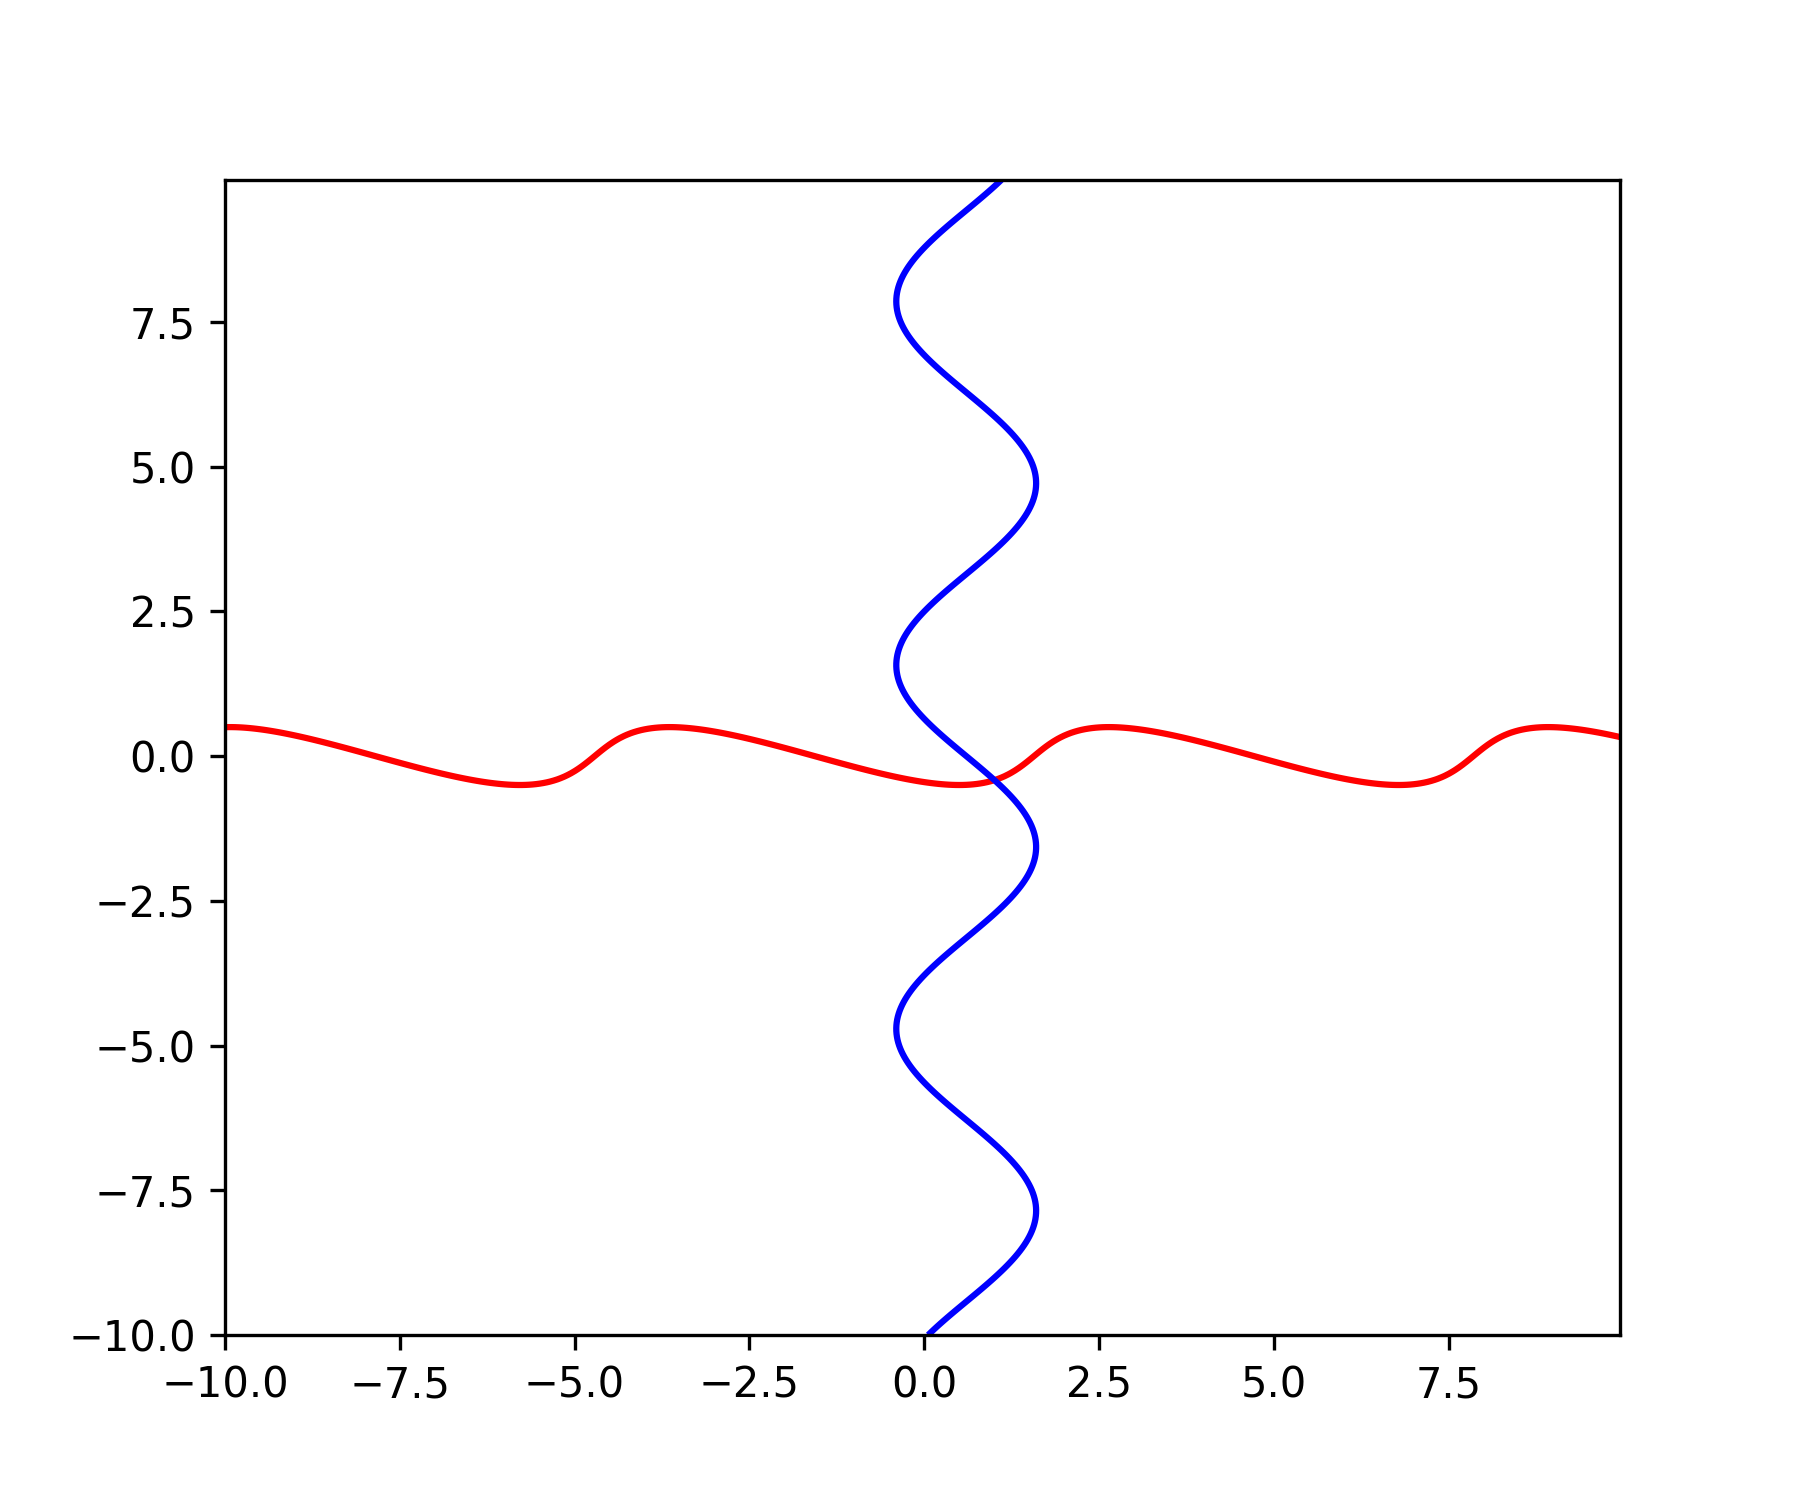
\includegraphics[width=0.49\linewidth]{../nonlinear_newton}
\end{figure}

Видно, что корень находится в пределах (0, 2.5) по оси x, и (-1, 1)  по оси y.

Результат работы программы:

\begin{minted}{text}
X1_my = array([ 1.00410184, -0.41599671])
Количество итераций: 4

X1_my = array([ 1.00410184, -0.41599671])
Количество итераций: 4

X1_scipy = array([ 1.00410184, -0.41599671])
X2_scipy = array([ 1.00410184, -0.41599671])
\end{minted}

\begin{figure}[h]
    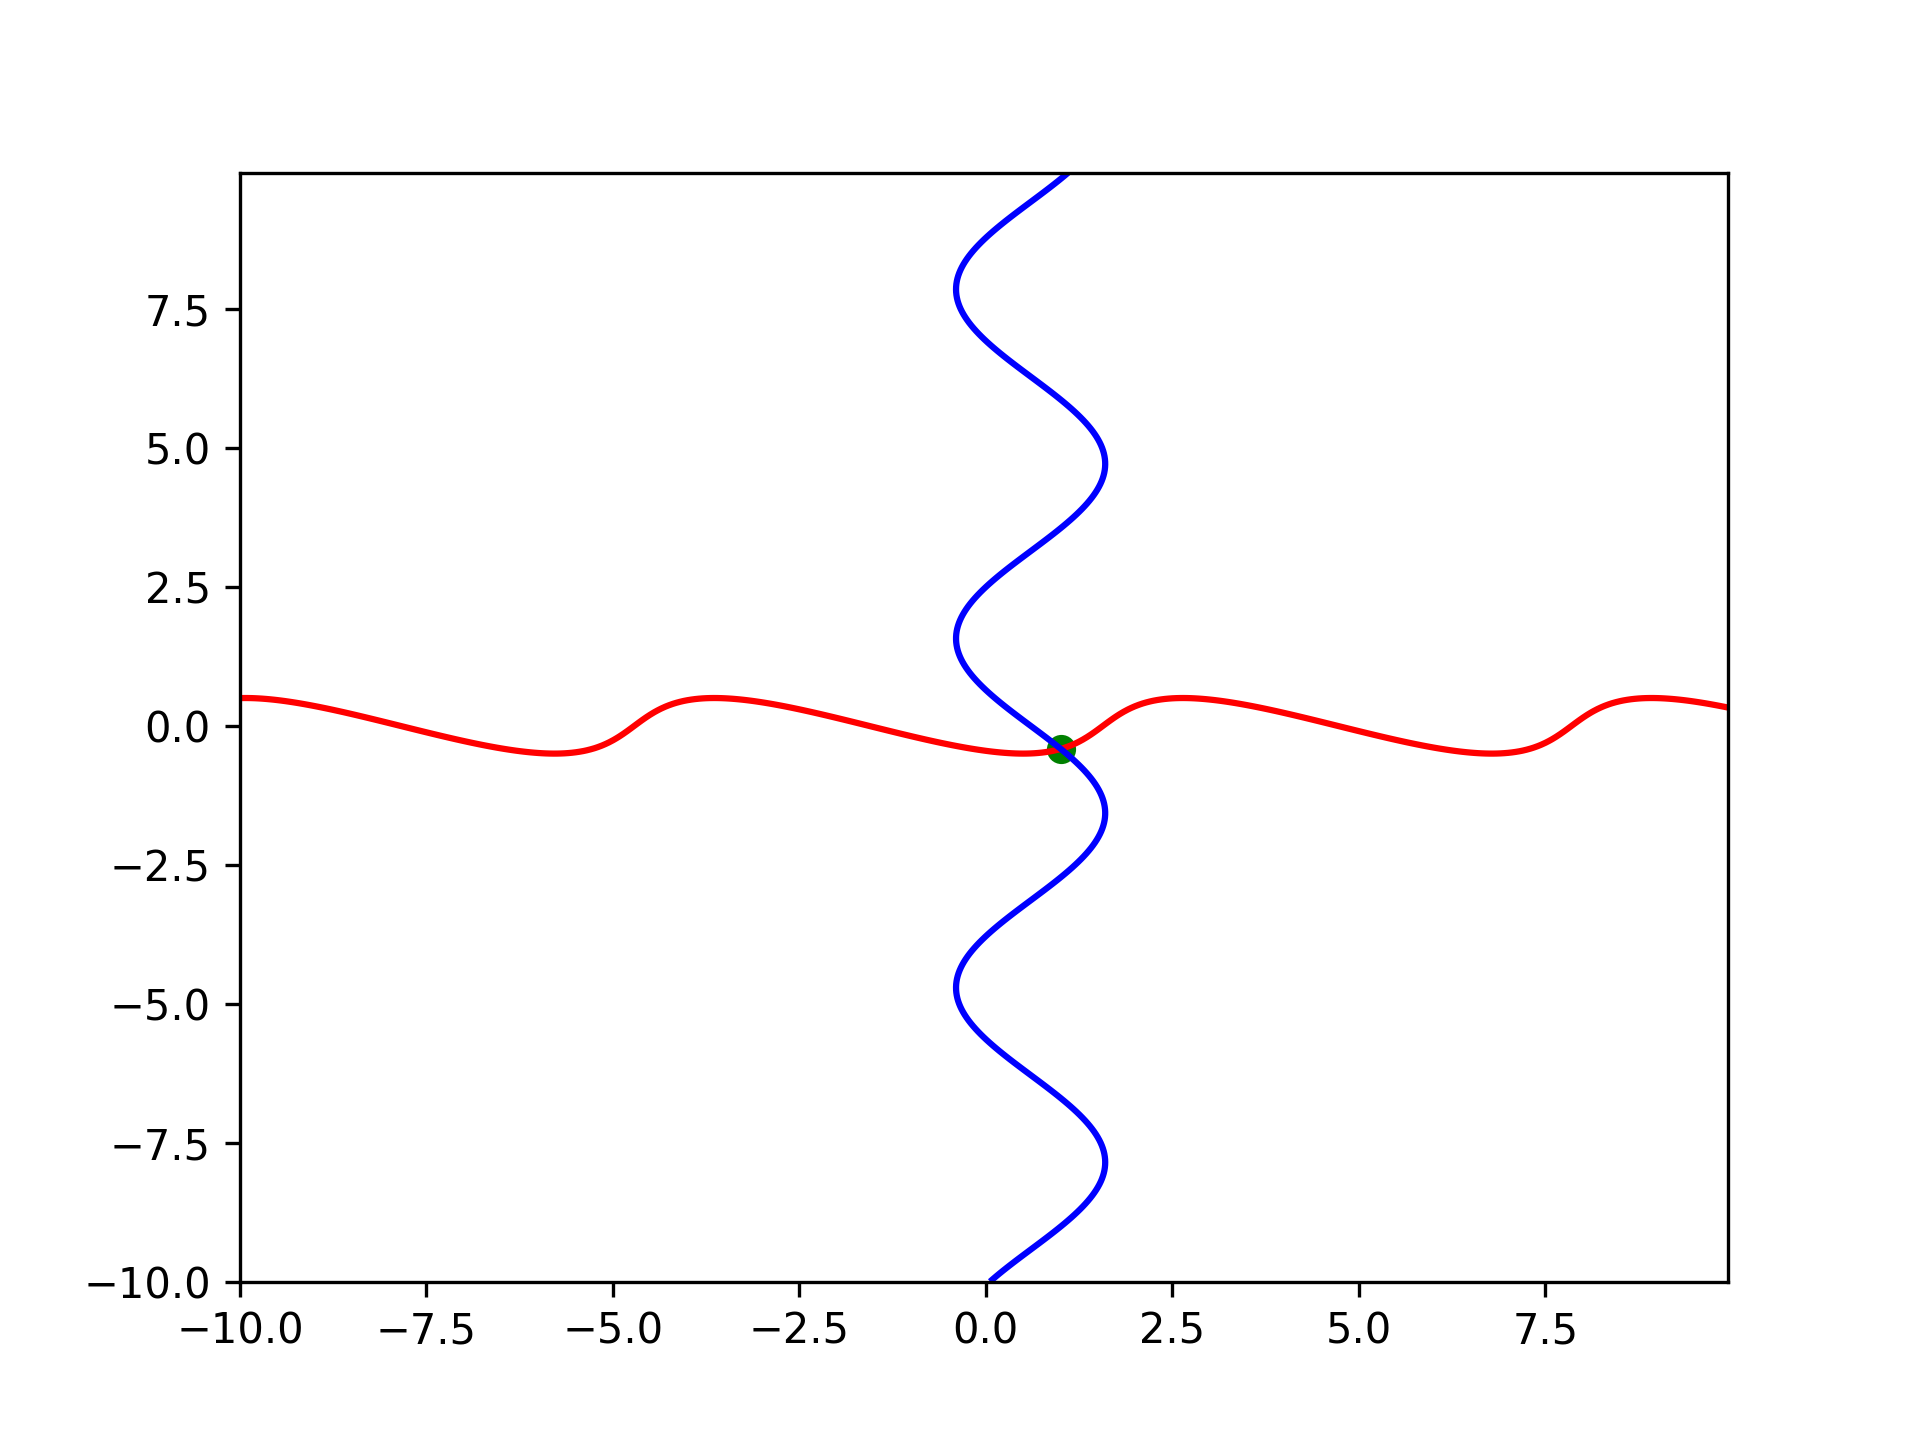
\includegraphics[width=0.49\linewidth]{../nonlinear_newton_with_point}
\end{figure}


\section{Расстояния от поверхности до точки (№ 4.5.2)}

\subsection{Формулировка задания}

Дана система уравнений $A x = b$. Найти решение системы с помощью метода Гаусса. Выполнить 10 итераций по методу Зейделя. Принимая решение, полученное с помощью метода Гаусса за точное, найти величину абсолютной погрешности итерационного решения.

\subsection{Код на Python}

\section{Метод Зейделя (№ 5.1.8)}

\subsection{Формулировка задания}

Дана система уравнений $Ax=b$. Найти решение системы с помощью метода Гаусса. Выполнить 10 итераций по методу Зейделя. Принимая решение, полученное с помощью метода Гаусса за точное, найти величину абсолютной погрешности итерационного решения.

1. Задать матрицу системы $A$ и вектор правой части $b$. Найти решение системы Ax=b с помощью метода Гаусса. 

2. Преобразовать систему $Ax=b$ к виду $x=Bx+c$, удобному для итераций. Проверить выполнение достаточного условия сходимости итерационных методов $\|B\|_\infty < \infty$

3. Написать программу-функцию zeid, решающую систему уравнений с помощью метода Зейделя, выполнить 10 итераций по методу Зейделя; взять любое начальное приближение. Принимая решение, полученное в п. 1 за точное, найти величину абсолютной погрешности итерационного решения.

4. Взять другое начальное приближение. Объяснить полученные результаты.

\subsection{Код на Python}

\insertMyCode{python3}{../zeid.py}

\subsection{Результаты}

\begin{minted}{text}
Решение методом Гаусса: [ 1.90875981 -2.36310552  4.49843079  1.62572378]

Начальная точка: [0. 0. 0. 0.]
Решение методом Зейделя: [ 1.90048704 -2.35749698  4.48910538  1.61896961]
Абсолютная погрешность: 0.00932540991025288

Начальная точка: [1. 1. 1. 1.]
Решение методом Зейделя: [ 1.90673816 -2.36173495  4.49615191  1.62407324]
Абсолютная погрешность: 0.0022788803781175204

Норма матрицы B: 0.996774193548387
\end{minted}

\section{Метод релаксации (№ 5.5.1)}

\subsection{Формулировка задания}

Дана система уравнений $Ax=b$, где $A$ – симметричная положительно определенная матрица. 
Найти решение системы с точностью $\varepsilon = 10^-5$ с помощью метода релаксации (для этого модифицировать функцию zeid из задачи 5.2, реализующую метод Зейделя). 
Определить экспериментально параметр релаксации $\omega$, при котором точность $\varepsilon$ достигается при наименьшем числе итераций. 
Построить график зависимости числа итераций от параметра релаксации.

\subsection{Код на Python}

\insertMyCode{python3}{../relax.py}

\subsection{Результаты}


\begin{minted}{text}

\end{minted}


\end{document}
